\documentclass{article}

\usepackage[scale=.75]{geometry}
\usepackage{soul}
\usepackage{siunitx}
\usepackage{url}
\usepackage{tikz}
\usetikzlibrary{decorations.pathreplacing,calligraphy,fit,matrix,calc,tikzmark}
\usepackage{fancyhdr}
\pagestyle{fancy}
\usepackage{fontspec}
\usepackage{unicode-math}
\setmainfont{TeX Gyre Adventor}
\setmathfont{TeX Gyre Bonum Math}
\usepackage{pgfmorepages}

\pgfpagesuselayout{2 on 1}

\lfoot{\textbf{Disclaimer}: The author accepts no warranty for the information in this document.
  The best way to check if a turkey is cooked is to use a meat thermometer.
}
\lhead{}
\chead{}
\rhead{}
\cfoot{}

\renewcommand\thesection{\Alph{section}}
\renewcommand*{\thefootnote}{\fnsymbol{footnote}}

\begin{document}
\section*{Keep a Sense of Proportion at Christmas}

Throughout, we assume that two objects of the same type have the same shape but can differ in overall size.
Under this assumption, if one direction (say, height) is scaled then all other directions (say, width and length) are scaled by the same amount.
Then any type of area is proportional to the square of any type of length, and any type of volume is proportional to the cube of any type of length.

In summary:

\begin{center}
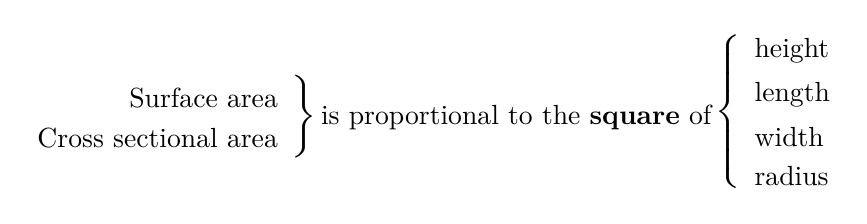
\begin{tikzpicture}
\node (sa) {Surface area};
\node[below left] at (sa.south east) (xa) {Cross sectional area};
\node[anchor=mid west] at ($(sa.south east)+(.3,0)$) (prop) {is proportional to the \textbf{square} of};
\node[anchor=south west] at ($(prop.east)+(.3,0)$) (len) {length};
\node[anchor=south west] at (len.north west) (ht) {height};
\node[anchor=north west] at (len.south west) (wd) {width};
\node[anchor=north west] at (wd.south west) (rad) {radius};
\node[inner sep=0pt,right delimiter=\},fit=(sa) (xa),node contents={}];
\node[inner sep=0pt,left delimiter=\{,fit=(ht) (rad),node contents={}];
\end{tikzpicture}

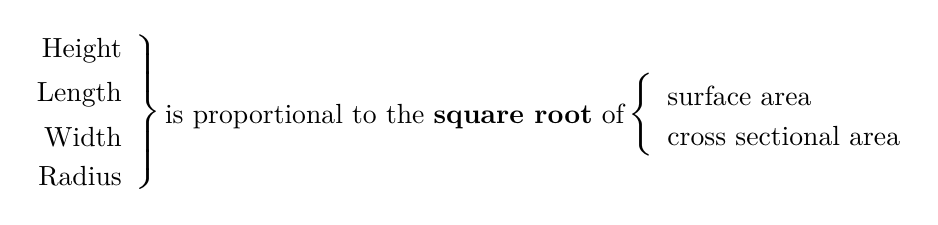
\begin{tikzpicture}
\node (len) {Length};
\node[anchor=south east] at (len.north east) (ht) {Height};
\node[anchor=north east] at (len.south east) (wd) {Width};
\node[anchor=north east] at (wd.south east) (rad) {Radius};
\node[anchor=mid west] at ($(len.south east)+(.3,0)$) (prop) {is proportional to the \textbf{square root} of};
\node[anchor=south west] at ($(prop.east)+(.3,0)$) (sa) {surface area};
\node[below right] at (sa.south west) (xa) {cross sectional area};
\node[inner sep=0pt,left delimiter=\{,fit=(sa) (xa),node contents={}];
\node[inner sep=0pt,right delimiter=\},fit=(ht) (rad),node contents={}];
\end{tikzpicture}

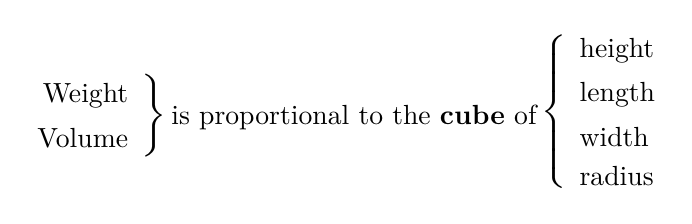
\begin{tikzpicture}
\node (wgt) {Weight};
\node[below left] at (wgt.south east) (vol) {Volume};
\node[anchor=mid west] at ($(wgt.south east)+(.3,0)$) (prop) {is proportional to the \textbf{cube} of};
\node[anchor=south west] at ($(prop.east)+(.3,0)$) (len) {length};
\node[anchor=south west] at (len.north west) (ht) {height};
\node[anchor=north west] at (len.south west) (wd) {width};
\node[anchor=north west] at (wd.south west) (rad) {radius};
\node[inner sep=0pt,right delimiter=\},fit=(wgt) (vol),node contents={}];
\node[inner sep=0pt,left delimiter=\{,fit=(ht) (rad),node contents={}];
\end{tikzpicture}

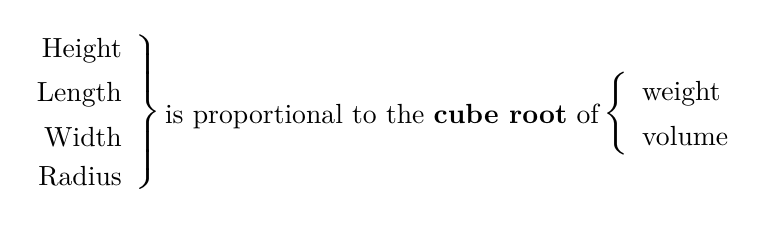
\begin{tikzpicture}
\node (len) {Length};
\node[anchor=south east] at (len.north east) (ht) {Height};
\node[anchor=north east] at (len.south east) (wd) {Width};
\node[anchor=north east] at (wd.south east) (rad) {Radius};
\node[anchor=mid west] at ($(len.south east)+(.3,0)$) (prop) {is proportional to the \textbf{cube root} of};
\node[anchor=south west] at ($(prop.east)+(.3,0)$) (wgt) {weight};
\node[below right] at (wgt.south west) (vol) {volume};
\node[inner sep=0pt,left delimiter=\{,fit=(wgt) (vol),node contents={}];
\node[inner sep=0pt,right delimiter=\},fit=(ht) (rad),node contents={}];
\end{tikzpicture}
\end{center}

\newpage
\lfoot{}
\setul{}{.3ex}
\section{It's All About the \st{Giving} Getting}


\begin{enumerate}
\item The number of lights needed to decorate a Christmas tree is proportional to the surface area of the tree.

\begin{enumerate}
\item If a \SI{2}{m} tree needs \num{250} lights, write a formula for the number of lights in terms of the height of the tree.
\item The Christmas tree in Trafalgar Square\footnote{Donated by the Norwegian Government} is about \SI{20}{m} tall.
How many lights would it take to decorate it?
\item I have \num{100} lights, how big a tree should I buy?
\end{enumerate}

\item The volume under the tree (available for presents) is proportional to the volume of the tree.

\begin{enumerate}
\item I can fit \num{20} presents under my \SI{2}{m} tree.
Write a formula for the number of presents that can fit under a tree in terms of its height.
\item How many presents would fit under the tree in Trafalgar Square?
\item How many presents would fit under my tree with \num{100} lights?
\end{enumerate}

\item In actual fact, the average size of present for my children is inversely proportional to their age.

\begin{enumerate}
\item My \num{9} year-old's presents average \SI{50}{cm} in length.
Use this to write down a formula for the average length of the present in terms of the child's age.
\item What's the average length of a \num{15} year-old's presents?
\item I've forgotten how old one of my children is.
The average length of their presents is \SI{42.5}{cm}.
How old are they?
\item My \num{90} year-old Grandmother is thinking of joining the digital revolution.
Assuming that the relationship between age and size of present still applies, what size smart phone can I buy for her?
\end{enumerate}

\item The quantity of pine needles dropped by a tree is proportional to its volume.

\begin{enumerate}
\item A \SI{2}{m} tree drops \num{20000} needles.
Write a formula for the number of needles a tree drops in terms of its height.

\item How many needles will the tree in Trafalgar Square drop?

\item One needle has a surface area of \SI{.1}{cm^2}.
Assuming that the presents under the tree have an average cross-sectional area of \SI{2000}{cm^2}, will I still be able to find the presents under the tree on Christmas morning?
\end{enumerate}
\end{enumerate}

\newpage
\section{Santa's Little Helper}

\emph{In these questions, use \num{3} significant figures of accuracy in your answers where appropriate.}

\begin{enumerate}
\item \emph{Twas the night before Christmas} was published in 1823 when the world population was approximately \num{1} billion.

The mean distance between dwellings is inversely proportional to the square root of the population.
In 1823, the mean distance was \SI{0.9}{km}.

\begin{enumerate}
\item Find a formula for the mean distance between dwellings in terms of the population.

\item In 2019, the world population is approximately \num{7.7} billion.
What is the mean distance between dwellings now?

\item Assuming that Santa is able to travel in such a way that on average, he travels the mean distance between dwellings, how far did Santa have to travel in 1823?
How far will he have to travel in 2019?

\item By careful use of time zones, Santa has \SI{30}{hrs} to deliver all the presents.
How fast did he have to travel in 1823?
How fast will he have to travel in 2019?
\end{enumerate}

\item The fact that Santa travels so quickly means that he is able to take advantage of relativistic effects to fit the presents on his sleigh\footnote{This is a load of rubbish.}.
The number of presents he has to deliver is proportional to the population size, so the length of his sleigh is proportional to the cube root of the population size.

In 1823, his sleigh was a normal \SI{5}{m}.

\begin{enumerate}
\item Find a formula for the length of the sleigh in terms of the population size.

\item How long does the sleigh need to be in 2019?
\end{enumerate}

\item The force needed to get the sleigh airborne is proportional to its weight, which is proportional to the number of presents, and thus is proportional to the world population.
In 1823, eight reindeer are mentioned in the poem.
How many reindeer does Santa need now?

For bonus points, what should Santa call them?

\item Climate change means that reindeer are getting smaller\footnote{This is true.}, so Santa has the opportunity of swapping his reindeer for smaller ones.
Santa works out that if he keeps the feed bill the same, the combined strength of the reindeer is inversely proportional to the length of an individual reindeer.

\begin{enumerate}

\item In 1823, a full sized reindeer was \SI{2}{m} and the combined strength of the reindeer was \SI{8}{rp}\footnote{\si{rp} stands for ``Reindeer power''.}.
Find a formula for the combined strength of the reindeer in terms of their length.

\item How long should the reindeer be that Santa uses in 2019 to pull the sleigh, given that he wants to keep the food bill the same?

\item How many reindeer will he need at this smaller size?
\end{enumerate}
\end{enumerate}

\newpage
\section{Cooking Up a Storm}

The time taken to roast a turkey, \(T\), consists of an initial time, \(a\), to bring the surface of the turkey to the right temperature, followed by the actual cooking time, \(t\).

Most advice for the roasting time of a turkey assumes that the initial time is fixed and that the actual cooking time, \(t\), is directly proportional to the weight, \(w\), of the turkey.

For each of the following websites, write a formula for the actual cooking time in terms of the weight.

Note that if \(t = k w\) then \(T = a + k w\) and the times given are for the total time, \(T\).

\begin{enumerate}
\item The site \url{http://britishturkey.co.uk} records the total time for a \SI{2}{kg} turkey as \SI{110}{mins} and for a \SI{3}{kg} turkey as \SI{130}{mins}.

% T = a + k w = 70 + 20 w

\item The site \url{http://www.bbcgoodfood.com} records the total time for a \SI{4}{kg} turkey as \SI{180}{mins} and for a \SI{6}{kg} turkey as \SI{260}{mins}.

% T = a + k w = 20 + 40 w

\item The site \url{http://www.bernardmatthews.com/how-to-cook-a-turkey} records the total time for a \SI{3}{kg} turkey as \SI{150}{mins} and for a \SI{7}{kg} turkey as \SI{230}{mins}.

% T = a + k w = 90 + 20 w

\end{enumerate}

In fact, the actual cooking time depends on how fast the heat gets to the turkey and so is proportional to the surface area of the turkey.
Since surface area is proportional to the \textbf{square} of the length, and the length is proportional to the \textbf{cube root} of the weight, surface area is proportional to the \textbf{square} of the \textbf{cube root} of the weight.
That is,
%
\[
  t \propto (\sqrt[3]{w})^2
  \]

For each of the above websites, assume that the actual cooking time taken to roast a small, \SI{2}{kg}, turkey is correct and use that to find a more accurate formula for the actual cooking time in terms of the weight.

Once a turkey is cooked, any more time that it spends in the oven simply dries it out.
A large turkey might weigh \SI{7}{kg}.
For each of the above websites, calculate how long a large turkey would spend drying in the oven.

\bigskip

Jamie Oliver's website makes the following recommendations:

\begin{tabular}{r@{-}r@{\si{kg} - cook }l@{ to }l@{ hours}}
\num{4}&\num{5}&\num{2.25}&\num{2.5} \\
\num{5}&\num{6}&\num{2.5}&\num{3} \\
\num{6}&\num{7}&\num{3}&\num{3.5} \\
\num{7}&\num{8}&\num{3.5}&\num{4} \\
\num{8}&\num{9}&\num{4}&\num{4.25} \\
\num{9}&\num{10}&\num{4.25}&\num{4.5}
\end{tabular}

Critique these timings.

\end{document}

\end{document}
